% EISI Final Paper 2014
% Jacob Lambert

\documentclass[twocolumn]{article}

% The geometry package assists with page formatting
\usepackage{geometry}
\geometry{letterpaper}

% Logo commands
\usepackage{doc}
\usepackage{amssymb}
\usepackage{amsmath}
\usepackage{relsize}
\usepackage{mathtools}

% URL formatting
\usepackage{url}

% Packages and definitions for graphics files
\usepackage{indentfirst}
\usepackage{amsfonts}
\usepackage{amsmath}
\usepackage{graphicx}
\usepackage{caption}

% Packages for box plot
\usepackage{amsbsy}
%\newcommand*{\clap}[1]{\hbox to 0pt{\hss#1\hss}}
\newcommand*{\mat}[1]{\boldsymbol{\mathrm{#1}}}
\newcommand*{\subdims}[3]{\clap{\raisebox{#1}[0pt][0pt]{$\scriptstyle(#2 \times #3)$}}}
\fboxrule=1pt



% Set the title, author, and date
\usepackage{authblk}
\title{Implicit Feedback Recommendation for Plant-pollinator Networks}
\author{Jacob Lambert} 
\affil{Department of Computer Science, Mathematics, University of Tennessee}
\date{}

%
% Document proper
%

\begin{document}

\maketitle

\abstract{
Examining and evaluating complex ecological communities is a popular study area of significant 
ecological value. Mutualistic plant-pollinator networks are an especially important community because
of the crucial role of pollinators in food production. However much is still unknown about the underlying
community structures of these networks and their stability under environmental perturbation. 
We present a method adapting recommender system collaborative filtering algorithms to the plant-pollinator
network in an attempt to quantify pollinator preferences and tendencies, and to predict future behavior. 
We apply an Implicit Feedback Matrix Factorization (IFMF) model originally developed for a TV show recommender
engine and discuss why this application is ecologically viable. Our results indicate that IFMF 
significantly outperforms a random-prediction model and is ripe for further development.
}

\section{Introduction}

\subsection{Plant-pollinator Networks}
Ecological communities can be very complex in nature. Several
types of relationships between species exist in communities, creating
layers of interdependence. The study of these relationships and their
effects on the community structures has significant ecological implications, both for montane meadows and the general human population\cite{bronstein2006evolution}.

Mutualistic relationships are especially interesting because of their
contrast with competition or predator-prey-based relationships.
Plant-pollinator networks are a
common and ecologically crucial example of mutualistic relationships.
\cite{ollerton2011many}. These mutualistic networks comprise a large
number of diverse plants and pollinators \cite{bascompte2007plant},
and they fill an important role in many land ecosystems.
Seventy-five percent of leading food crop production depends on
pollinators \cite{klein2007importance}.

Despite the critical environmental role of plant-pollinator networks,
there exist many open questions regarding the community structure,
inter-species dependencies of these networks, and especially network stability under environmental
perturbation such as climate change \cite{hegland2009does}.

Mutualistic networks easily lend themselves to bipartite graph representation because of their dualistic nature.
We can abstract the plant-pollinator network into a bipartite graph by treating the 
plants as one partition and the pollinators as another. Many analytical methods and algorithms
exist specifically for bipartite networks\cite{bipartite}, making the abstraction useful for uncovering
hidden structures within the plant-pollinator network.
\begin{figure*}
  \caption{Bipartite representation of plant-pollinator networks. Plants are listed in the upper trophic level, and
  pollinators are listed on the bottom level.}
  \centering
  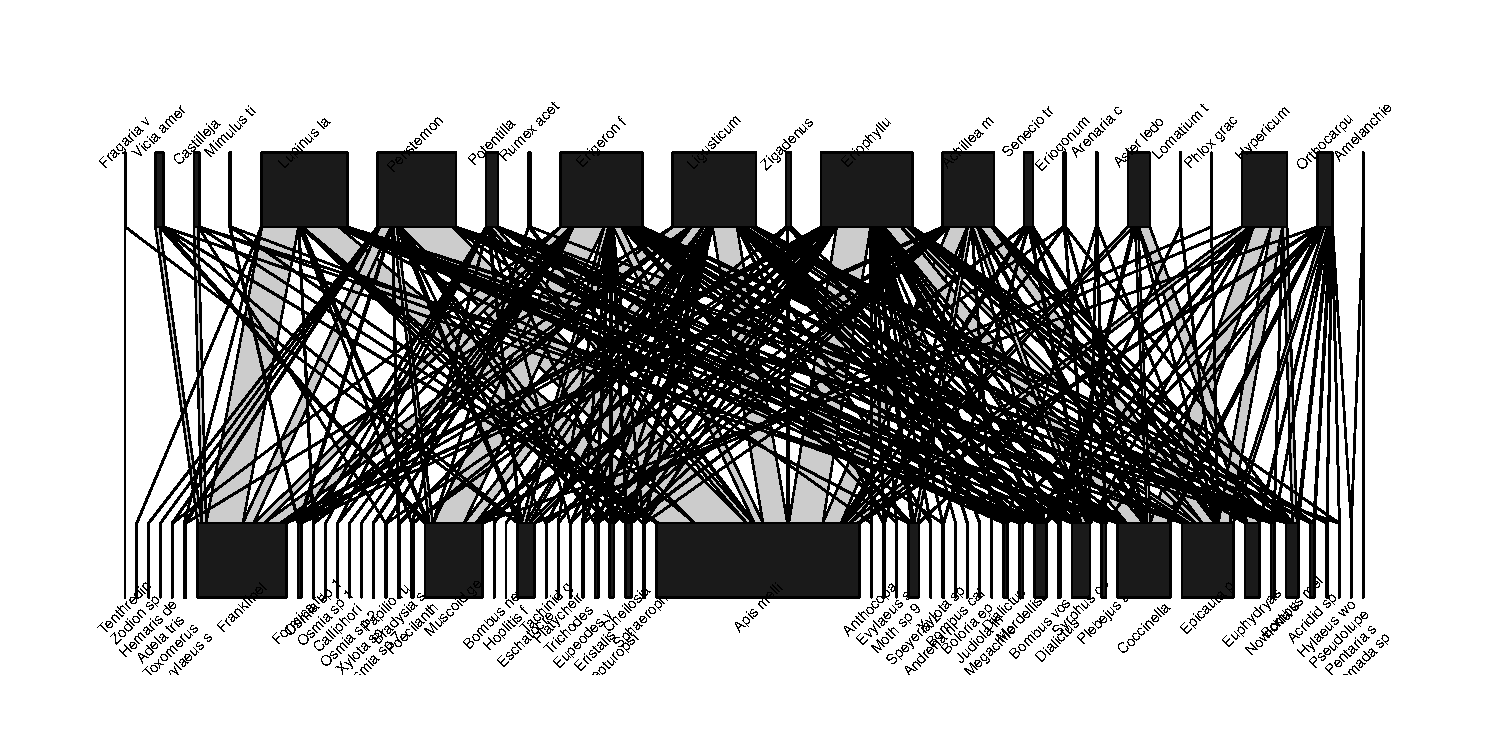
\includegraphics[scale=0.65]{bipartite.pdf}
\end{figure*}

\subsection{Recommender Systems, Collaborative Filtering, and Implicit Feedback}
Recommendation systems have immense utility in commercial applications. 
Numerous systems involving users and products, for example movie and 
music-streaming applications such as Netflix and Pandora, employ recommender systems
to recommend new products to users. Similarly, many product and consumer systems 
like Amazon use recommender systems to calculate which new products a user may 
wish to purchase.
These systems attempt to recommend products based on that specific user's purchase
history or user-entered preferences. 

Recommender systems with a large number of users and 
products can exercise 
collaborative filtering methods instead of storing specific  user preferences.
Collaborative filtering utilizes information from 
many different users to calculate preferences for product-item pairs of one specific user. 
These systems are normally equipped with a rating system, 
where users explicitly rate items either positively or negatively. For example, a 1-star rating
may indicate that the user did not enjoy an item, while we can infer from a 5-star rating that
the user did enjoy the item.

However, not all algorithms require explicitly 
defined user ratings. One method developed \cite{hu2008collaborative} is 
designed specifically for implicit feedback. 
Unlike explicit feedback such as ratings, implicit feedback is an 
indirect measure of user preferences based on behaviors. For example, 
implicit feedback can be gathered from a system involving 
users and television programs. Normally users have no way of explicitly
rating a television program. However, we can 
infer from their behavioral patterns that a user may prefer a certain 
program if he or she watches it several times. Hu, Koren, and Volinski's method was specifically developed for a TV show 
recommender engine\cite{hu2008collaborative}.

Although implicit feedback systems are similar to explicit systems, 
there exist important distinctions. Because users never explicitly rate 
products, it is difficult to infer which items a user does not like. 
For example, a user may not watch a certain show for several reasons, 
including time conflicts or lack of knowledge about the program. 
Similarly, we cannot always infer that a user enjoys a show because he or 
she watched it.  Perhaps the user was away from the television at that 
time or watching the show preceding a favorite program.
       
For this reason, unlike explicit feedback systems where the numerical 
value of a user-item interaction is an indication of preference, the 
numerical value in implicit feedback systems indicates a confidence of 
the interaction. In the TV show recommendation engine, the numerical
values represent the number of times of a user watched a certain program.
For implicit systems, a large value does not inherently imply a 
higher preference, only a higher frequency of interaction. 
Therefore, large values in implicit feedback systems indicate a higher confidence
in a user's preference for an item. 

The implicit feedback system developed by Hu et al. (2008)\cite{hu2008collaborative} is appropriate for 
application to plant-pollinator networks. Like the TV show scenario, we have 
no way of observing any explicit rating of plant preferences by pollinators. 
However, a high-frequency interaction grants a degree of confidence for a pollinator's
preference for a plant.
Similarly, like the TV show recommendation engine, we don't immediately associate a lack of interaction
with a negative preference. Competition can be seen as a form of time conflict, which may result
in a pollinator not visiting a plant they prefer. Also, we hypothesize that many interactions
may go unobserved due to weaknesses in data collection methods.
\begin{figure}
  \caption{Graphical representation of the plant-pollinator interactions. The shade of yellow indicates the 
  magnitude of observations of the interaction between that specific plant and pollinator.}
  \centering
  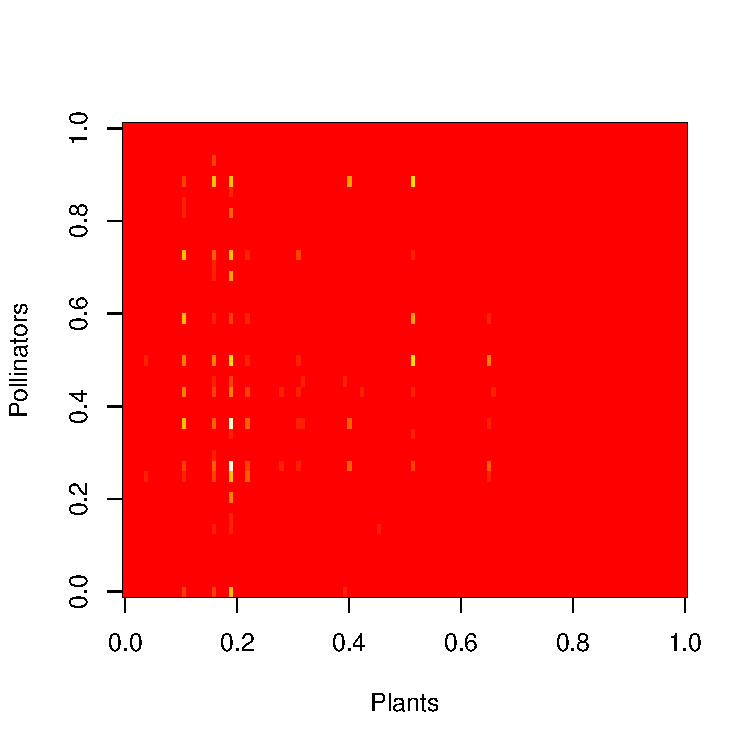
\includegraphics[scale=0.5]{fullMat.pdf}
\end{figure}

We hypothesize that by applying an implicit feedback recommender system to the plant-pollinator network,
we can uncover hidden truths about the structure of the network. By calculating which plants would be
recommended to the pollinators, we can attempt to detect which interactions have yet to be observed but 
are likely to occur. Also,
in the event of environmental changes or extinction of certain species, we can predict  shifts in
plant-pollinator interactions based on the different types of plants recommended to each pollinator.

\section{Methods}

\subsection{Data Collection}
The data used in this study was collected during the summer months of
2011  within H.J. Andrews Experimental
Forest, central Cascades Oregon. Within the forest, several different complexes were
defined, each having three separate but geographically close montane
meadows.

Each of these meadows are uniquely classified within the data-set.
Within these meadows, we sampled from two transects of 3-meter square
plots. These transects are separated by 25 meters, and each transect
contains 5 subplots separated by 15 meters. The subplots are numbered 1-10 
according to their associated transect and position within the transect.
This configuration of
plots and transects is assumed to be representative of the dominant
characteristics of each meadow \cite{pfeiffer2012influence}.

\subsubsection{Field Methods}
Data recording was conducted on an approximately weekly basis for each
meadow, which consisted of a sampling of flower vegetation levels and
pollinator activity. Our study solely relies on the pollinator activity
data.

To record pollinator activity, each plot of each meadow was surveyed for
a 15  minute interval, or watch. Any time a potential pollinator made contact with
the reproductive systems of a flower in antithesis, an interaction between
the specific pollinator and flower species was recorded. If a plant or pollinator
was not immediately identifiable, a sample was collected for later
identification.

The time, weather, plot number, and flower abundances were also
recorded for each 15-minute watch. For a more detailed description of the
data collection methodology and ecological justification for design
choices, see \cite{pfeiffer2012influence}.

\subsubsection{Laboratory Methods}
Any unidentifiable flower was either sampled and or photographed
for identification. To identify unknown flowers, we referenced
\cite{mackinnon2004plants}. We then cross-referenced
successful identifications with the H.J. Andrews botanist-conducted
flower surveys and data collected in previous years.

We attempted to collect a sample of each pollinator that could not be
identified by sight. However, because of the vagility of the pollinators,
many
entries in the data set are only accurate to a certain degree of
taxonomic precision.

Once sampled, we pinned each pollinator with an associated identification
number, along with data about where and by whom the pollinator was
collected. Although we were confident in identifying some abundant
species, many of our samples were forwarded to Oregon State University entomologist
Andy Moldenke for accurate classification. We entered our data systematically, associating each observed interaction with an observer, date, time, weather, location,
and the involved species. 
\begin{table*}[!htbp] \centering
  \caption{Simplified example of recorded data for plot watches. Complexes can be identified based on the meadow code.}
  \begin{tabular}{@{\extracolsep{1pt}} lrcccc}         
    \\[-1ex]\hline   
    \hline \\[-1ex]   
    MEADOW & DATE & OBSERVER &  PLOT & PLTSP\_NAME & VISSP\_NAME \\                                                 
    \hline \\[-1ex]  
    CPM & 7/1/2014 & RD & $1$ & Zigadenus venenosus & Bombus mixtus \\               
    LM & 6/30/2014 & JL & $3$ &  Zigadenus venenosus & Bombus mixtus \\             
    LB & 7/10/2014 & RM & $7$ &  Senecio triangularis & Apis mellifera \\             
    CPB & 7/3/2014 & IP & $9$ & Erysimum asperum & Bombylius major \\              
    \hline \\[-1ex]  
  \end{tabular} 
\end{table*} 

\subsection{Implicit Feedback System}

\subsubsection{IFMF Implementation}

The implicit feedback matrix factorization model (IFMF) was implemented in the R programming language and is detailed in \cite{hu2008collaborative}. This method applies matrix 
factorization to decompose the original matrix into two latent factors, one for users and one for items. 

Latent factor models attempt to explain ratings or preferences by characterizing items and users
on a set of factors inferred from the rating or preference patterns \cite{koren2009matrix}.  For example, 
in a music recommendation system matrix factorization,
the product latent factor may measure more obvious dimensions like genre, era, instrumental type, or typical audience.
For our plant-pollinator network, the plant factor may measure physical dimensions such as plant genus, size,
color, or flower size, while the pollinator factor may represent pollinator family or genus, flight speed, mass,
or even proboscis length.

The matrix targeted for decomposition, $r_{ui}$, is the observation matrix.
The rows correspond to $u$ users, or pollinators, and the columns correspond to $i$ items, or plants. 
Each $r_{ui}$ entry corresponds to the number of interactions observed between $u$ and $i$ during
the observation period.

\begin{figure}
  \caption{Visual of matrix decomposition. $r$ refers to the observation matrix, $X$ refers to the pollinator factors, and $Y$ refers to the plant factors}
  \[
    \framebox[2.5cm]{\clap{\raisebox{0pt}[1.5cm][1.5cm]{$\mat r$}}\subdims{-2.5cm} m n} =
    \framebox[1.5cm]{\clap{\raisebox{0pt}[1.5cm][1.5cm]{$\mat X$}}\subdims{-2.5cm} m f} \ 
    \framebox[2.5cm]{\clap{\raisebox{5mm}[1.5cm]{$\mat Y$}}     \subdims{-1cm} f n}
  \]

\end{figure}

In addition to the matrix of interactions, we also generate a binary matrix $p_{ui}$, which indicates
the initial observed preferences of each pollinator $u$ to plant $i$.
\begin{displaymath}
  p_{ui} = \left\{
    \begin{array}{lr}
      1 & : r_{ui} > 0\\
      0 & : r_{ui} = 0
    \end{array}
  \right.
\end{displaymath}

If $p_{ui} = 1$, then we believe that pollinator $u$ has a preference for plant $i$. If $p_{ui} = 0$ then we
have no indication of the preference for pollinator $u$ to plant $i$. However, these preferences are 
associated with a specific confidence. We measure the confidence of preferences with $c_{ui}$, a logarithmic
reduction of $r_{ui}$.

\begin{equation}
  \label{eq:1}
  c_{ui} = 1 + \alpha\log (1 + r_{ui}/\epsilon)
\end{equation}
Both $\alpha$ and $\epsilon$ are variables that can be adjusted during the training process. Value
$\alpha = 40$ was found to produce good results when applied to our testing and training data sets,
while small values such as $\epsilon = 10^-8$ are appropriate
\cite{hu2008collaborative}.

We now need to calculate a latent factor vector of length $f$: $x_u \in \mathbb{R}^f$ for pollinators and 
$y_i \in \mathbb{R}^f$ for plants. Appropriate values for $f$ can be determined by training.
Once calculated, the predicted preferences are assumed to be the inner products: $\hat{p}_{ui} = x^{T}_{u}y_{i}$

To calculate the latent factors, we must minimize the following cost function:
\begin{equation}
  \label{eq:2}
  \underset{x_{*}, y_{*}}{\text{min}}
  \underset{u,i}{\mathlarger{\sum}}
  c_{ui}(p_{ui} - x^{T}_{u}y_{i})^2 + \lambda\left( 
  \underset{u}{\sum}|x_{u}|^2 + \underset{i}{\sum}|y_{i}|^2
  \right)
\end{equation}

An efficient optimization strategy evolves from alternatively fixing one of the factors while recomputing 
the other.  After a sufficient number of sweeps, the factors stabilize on an optimal solution \cite{hu2008collaborative}.

With the $n$ item factors fixed, we can gather them into an $n \times f$ matrix $Y$. Also, for each user $u$ we can
define an $n \times n$ matrix $C^u$, where $C^u_{ii} = c_{ui}$ and a vector of preferences $p(u) \in \mathbb{R}^n$.
Differentiation leads to a solution for the user factors $x_{u}$ that minimizes the cost function $\ref{eq:1}$\cite{hu2008collaborative}. 
\begin{equation}
  \label{eq:3}
  x_{u} = (Y^{T}C^{u}Y + \lambda I)^{-1}Y^{T}C^{u}p(u)
\end{equation}

With the $m$ user factors fixed, we can now use the same technique to compute the $y_i$ item factors.
\begin{equation}
  \label{eq:4}
  y_{i} = (X^{T}C^{i}X + \lambda I)^{-1}X^{T}C^{i}p(i)
\end{equation}

The $\lambda$ parameter prevents over fitting of the model and can be tuned by appropriate training.
The running time of these equations is $O(f^{2}N + f^{3}m + f^{3}n)$ where $N$ is the number of 
non-zero observations\cite{hu2008collaborative}. This running time is linear with respect to the size of the inputs, $m$ pollinators
and $n$ plants. 

After performing an appropriate number of sweeps for the factors to stabilize, it is possible to construct
the matrix $\hat{p}_{ui} = x^{T}_{u}y_{i}$, where $\hat{p}_{ui}$ represents the predicted preference of pollinator $u$
for plant $i$.

\subsubsection{Training and Testing}

In order to tune training variables ($f$, $\lambda$, $\alpha$, $\epsilon$), appropriate training and testing sets
are required. For the TV show recommender engine, several months of complete data were used to train these parameters
of IFMF, and several disjoint months of complete data were used to validate the training.

For our plant-pollinator network, we have split the data collected during the summer of 2011 into four sets,
determined by plot number. We felt that division at the plot level was more appropriate than the meadow or complex
level. Due to geographical differences in the meadows and especially complexes such as elevation, temperature, 
sun exposure, and soil moisture, some species of plants and pollinators are not present in all meadows and complexes.
Because we can only make predictions about plants and pollinators that are present in both the training and testing
data sets, we chose to divide the sets by plot so that a maximal number of species from all complexes and meadows are present in both
the training and testing data sets.

The sub training matrix $r^{s}_{ui}$ consists of plots 2, 5, and 8 across all meadows and complexes and is used along 
with the validation matrix $r^v_{ui}$ consisting of plots 3, 6, and 9 in order to tune parameters. Once the 
parameters have been tuned appropriately, the training matrix $r_{ui}$ is redefined as a combination of 
$r^s_{ui}$ and $r^v_{ui}$, consisting of plots 2, 3, 5, 6, 8, and 9. The testing matrix $r^t_{ui}$ consists of the
remaining plots, 1, 4, 7, and 10. 
\begin{table}[!htbp] \centering
\caption{Organized explanation of dataset partitions}
\begin{tabular}{@{\extracolsep{1pt}} lcc}
\\[-1ex]\hline
\hline \\[-1ex]
Matrix & Notation & Plots \\
         \hline \\[-1ex]
         subtrain & $\mathlarger{r^s_{ui}}$ & 2,5,8\\                           
         validate & $\mathlarger{r^v_{ui}}$ & 3,6,9\\
           train    & $\mathlarger{r_{ui}}$   & 2,3,5,6,8,9\\
           test     & $\mathlarger{r^t_{ui}}$ & 1,4,7,10\\
           \hline \\[-1ex]
           \end{tabular}
           \end{table}

For validation of the method and tuning of parameters, we implemented a 
mean percentile rank (MPR) measure. In contrast to most explicit feedback
recommender systems, we are not able to track user reactions to 
recommendations. Therefore, precision-based metrics are less appropriate
because they require knowledge of undesirable products 
\cite{hu2008collaborative}.

However, observations are indicative of preference, so recall-oriented 
measures such as MPR are appropriate\cite{hu2008collaborative}. Let 
$rank_{ui}$ represent the percentile-ranking of a plant $i$ from the
list of prepared plants for pollinator $u$. That is, $rank_{ui} = 0$ 
indicates a highly recommended plant, while $rank_{ui} = 1$ indicates
an undesirable plant for pollinator $u$. We then calculate the MPR as follows:
\begin{equation}
  \overline{rank} = \dfrac
    % num
    {\sum_{u,i}r^t_{ui}rank_{ui}}
    % den
    {\sum_{u,i}r^t_{ui}}
\end{equation}

We tune the parameters by attempting to minimize the value of 
$\overline{rank}$ (values of $\overline{rank} > .5$ indicates the 
algorithm performs worse than at random)\cite{hu2008collaborative}. 

\section{Preliminary Results}

We first tested several configurations of parameters. See table 3 on page~\pageref{parest}. 
As a starting point, we used the parameters
found to perform well for the TV show recommender engine. A more-exhaustive parameter search would involve a 
grid search or Bayesian optimization technique. From the configurations tested, values of $\alpha = 20$, 
$\epsilon = 10^-8$, $\lambda = 0.5$, $f = 30$ were found to produce good results in the sub training and sub testing data sets using the MPR metric.

A lower bound $lb$ was introduced for performance comparison. The $lb$ is calculated by providing the ranking 
algorithm the exact ranks of the testing matrix. An upper bound is also introduced in a similar manner by 
inverting the ranking used in $lb$.  

Finally, we graph a comparison of the training matrix $r_{ui}$ and $\hat{p}_{ui} = x^{T}_{u}y_{i}$, the calculated
preferences determined by IFMF from $r_{ui}$. See figure 4 on page~\pageref{compgraph}. Because of the differences in scaling, the values in the graph of
$\hat{p}_{ui}$ exponentiated, allowing a more representative visualization of the differences in values. 

We can see in figure 4 that the training matrix differs significantly from the training matrix. That is, by applying IFMF we can see
many new potential plant-pollinator interactions. The goal is to calculate or estimate the validity of these new interactions.

\begin{table*}[!htb] \centering
\label{parest}
\caption{Examples of configurations of variables used to tune the algorithm. Lower values of $\overline{rank}$, shown
  in the right columns, represent better algorithm performance. The actual validation test, represented by $(r^s,r^v)$ 
    is compared against a lowerbound $lb$, an upperbound $ub$ and $random$, the expected result of a random 
    assignment of preference rank. Finally, the tuning of each parameter set is applied to the larger training
    and final testing data sets, $(r_{ui}, r_{ui}^t)$.}
  \begin{tabular}{@{\extracolsep{1pt}} ccrc|ccccc}
    \\[-1ex]\hline
    \hline \\[-1ex]
      & & Parameters & & & & $\overline{rank} = MPR(train, test)$  & & \\
    \hline \\[-1ex]
      $\alpha$ & $\epsilon$ & $\lambda$ & $f$ & $ub$ & $lb$ & $(r^s,r^v)$ & $random$ & $(r_{ui},r^t_{ui})$ \\
    \hline \\[-1ex]
     $1$   & $10^-8$ & $0.1$  & $5$  & $0.932$ & $0.068$ & $0.288$ & $0.500$ & \\ 
     $20$  & $10^-8$ & $0.1$  & $5$  & $0.932$ & $0.068$ & $0.348$ & $0.500$ & \\ 
     $20$ & $10^-8$ & $5$     & $20$ & $0.932$ & $0.068$ & $0.282$ & $0.500$ & \\ 
     $20$ & $10^-8$ & $0.5$   & $30$ & $0.932$ & $0.068$ & $0.245$ & $0.500$ & $0.249$\\ 
    \hline \\[-1ex]
  \end{tabular}
\end{table*}

\begin{figure*}
  \label{compgraph}
  \caption{Comparison of the training matrix (left) $r_{ui}$ with the generated recommendation preferences 
  $\hat{p}_{ui} = x^{T}_{u}y_{i}$ (right). }
  \centering
  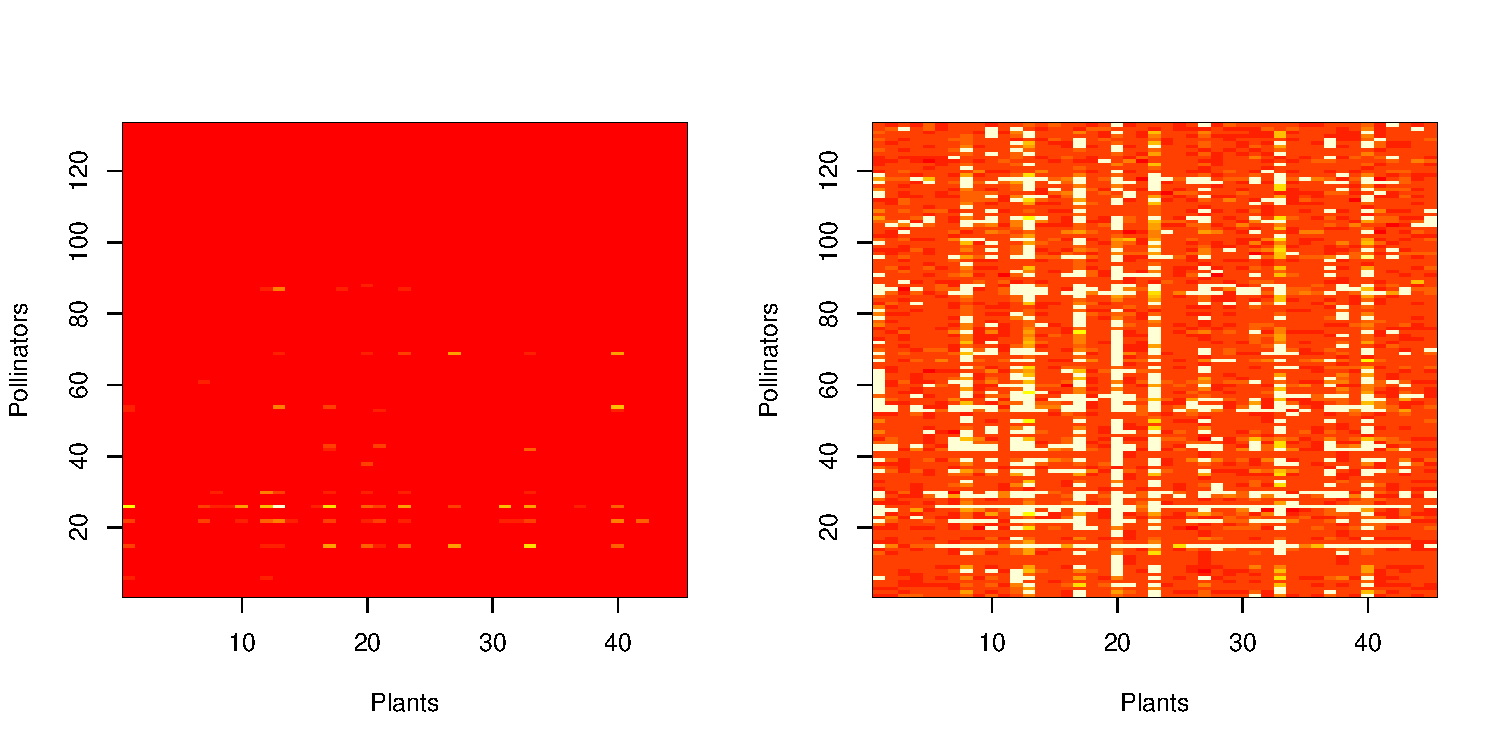
\includegraphics[scale=0.4]{train_pf.pdf}
\end{figure*}

\section{Discussion and Future Work}

\subsection{Discussion}
The TV show recommender engine recommends those shows not previously 
watched with the highest computed preferences to the user. In our 
plant-pollinator scenario, we attempt to predict which observations 
we may have missed in our data-collection.

IFMF with appropriately-tuned parameters out-performs both the upperbound worst case model and the random model. 
The most sensitive parameter seems to be $f$, the number of factors. While increasing the number of
factors decreases the value of $\overline{rank}$, an excessively large number of factors compromises the 
ecological interpretability of the assignment of latent factors. 

Our current metric for ranking the algorithms relies solely on that algorithm's ability to predict
from the training set the rank of all plant-pollinator interactions in the testing set. However, it is 
not difficult or 
interesting to predict that a pollinator will revisit a plant in the testing set that it has previously 
visited in the training set. Therefore, the next step in algorithm construction is to only consider plants in the
testing set that are not present in the training set.

\subsection{Future Work}

Although separating training and testing sets seems ecologically valid
in most instances, certain pollinators visit very few new plants from
the sub training set ($r^s_{ui}$) to the validating set ($r^v_{ui}$). 
Because it can be difficult to accurately predict recommendations on 
such a specific scale, the variable parameters ($f$, $\lambda$, $\alpha$, 
$\epsilon$) may be ill-tuned for these pollinators. 

One suggested solution involves intentionally removing observed
interactions from the sub training set. This will result in a higher number
of new interactions in the validation set, potentially leading to more
accurate and useful training parameters. Additionally, once we feel that
the data from the years 2012-2014 have been appropriately prepared, we 
can redefine our training and testing sets to include these interactions.

The TV show recommender engine was compared against several other
recommendation methods, including a neighborhood and popularity-based 
model. IFMF outperformed both models when applied to the TV show
dataset. It would be interesting to compare the performance of these
algorithms, especially the popularity-based model, to our 
plant-pollinator dataset. 

The popularity-based model recommends the most popular shows to 
all users. For its simplicity, this model performed surprisingly well 
when applied to the TV show dataset, perhaps because users are drawn
to popular shows by both preferences and word-of-mouth/social pressures.
I hypothesize that the popularity-based model would also perform well
on our plant-pollinator network. From anecdotal intuition formed during
data collection, many different types of pollinators are drawn toward 
a small set of flowers, perhaps because of their abundance and nectar
rewards.

Additionally, a comparison of the specific species differences between
IFMF and a popularity-based model could have interesting ecological
implications, such as a connection between physical pollinator traits and
a calculated recommendation for non-popular plants. 

Lin et al. expand upon the framework IFMF to include negative implicit 
feedback \cite{lin2014signals}. IFMF2 is developed for a crowdsourcing
application, where users are recommended jobs. Interestingly, IFMF2 
accounts for the availability of jobs, and interprets a lack of
interaction between a user $u$ and a job $i$ in the presence of 
high-availability of $i$ as negative feedback from $u$ to $i$.

If applied to our plant-pollinator dataset, IFMF2 would assume that
a lack of interaction from a pollinator $u$ with a plant $i$ when 
presented with an abundance of plant $i$ indicates a negative preference
from pollinator $u$ for $i$. It is safe to assume in the crowdsourcing
dataset the absence of an observation between $u$ and $i$ implies 
no interaction occurred, which justifies an application of negative 
implicit feedback\cite{lin2014signals}. However, in the plant-pollinator
network, an 
unobserved interaction between a plant and pollinator does not 
necessarily imply no interaction occurred.

It would be interesting to compare the results and performance of
IFMF and IFMF2, which could validate or invalidate the ecological
assumption that lack of observed interactions between a pollinator and
an abundant plant implies that the pollinator does not prefer that plant.

Physical traits of the pollinators could also be an interesting metric
for comparison with the recommendations of IFMF. Andy Moldenke of Oregon 
State University has developed a model indicating the probability of 
a plant-pollinator derived from ecological intuition and rigorous field
experience. See figure 5 page~\pageref{aMx}\cite{moldenke2014pollination}.
\begin{figure}
  \label{aMx}
  \caption{Ecologically derived probabilities for plant-pollinator interactions}
  \centering
  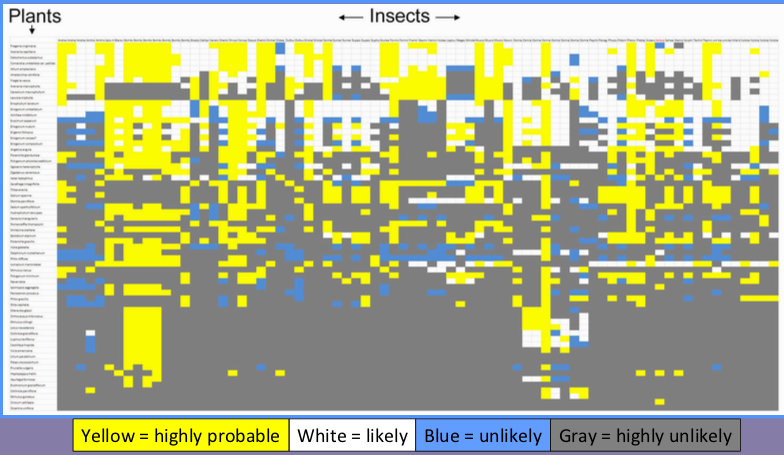
\includegraphics[scale=0.25]{AndyMx.png}
\end{figure}

\section{Conclusion}
We have collected data detailing the flower abundance and 
plant-pollinator interactions of montane meadows in H.J. Andrews 
Experimental Forest, Western Cascades Oregon.

We have a method that applies an Implicit Feedback
Matrix Factorization algorithm, originally developed for a TV show 
recommender engine, to our plant-pollinator dataset. We have shown that
the concept of collecting implicit feedback from users in the TV show 
recommender engine is analogous in many ways to our observations 
of plant-pollinator interactions.

We have also shown that IFMF applied to our plant-pollinator dataset
performance $(0.249)$ is significantly better than an expected 
random ranking model $(0.500)$. We have also presented several possible
improvements for our method, including comparisons to other popular
models. Ultimately, we have shown that the 
novel application of IFMF recommendation system collaborative filtering
algorithms to mutualistic plant-pollinator networks takes into account
many ecological viability considerations and is a research area worthy of future study.

\section{Acknowledgments}
I would like to thank the NSA for providing funding for Oregon State's 2014 EISI REU program, 
and Oregon State for hosting the REU program.

I would also like to think Julia Jones, Tom Dietterich, Jorge Ramirez, Andy Moldenke, and Rebecca Hutchinson for being excellent faculty
mentors during the program. Similarly, I want to thank Eddie Helderop and Veera Pfeiffer for their on-site mentorship.

Finally, I want to thank all of the other EISI 2014 REU students for their encouragement and insight during this project.
% Generate the bibliography
\nocite{Hmisc}
\nocite{R}
\nocite{dormann2009indices}
\bibliographystyle{plain}
\bibliography{EISI_Report}

\appendix
\section{Appendices}

For my R code and derived data sets, contact jlmabe17@vols.utk.edu

\end{document}
